%============================================================
%     Group Meeting Report Template — Computational Imaging
%============================================================
\documentclass[15pt]{beamer}
\makeatletter
\makeatother

%======================== packages & settings ========================
\usepackage{amsmath, pifont, bookmark, tabularx, booktabs, adjustbox, graphicx, caption, subcaption, listings, color, tikz}
\usetikzlibrary{arrows.meta,positioning,shapes.geometric,shapes.misc,fit,calc,decorations.pathreplacing}
\usepackage{hyperref}
\hypersetup{colorlinks=true,linkcolor=blue,urlcolor=blue}
\usepackage{array}
\newcolumntype{P}[1]{>{\raggedright\arraybackslash}p{#1}}

%======================== theme & fonts ========================
\usetheme{Montpellier}
\renewcommand{\familydefault}{\sfdefault}

% TOC numbered
\setbeamertemplate{section in toc}[sections numbered]
\setbeamertemplate{subsection in toc}[subsections numbered]

% footer
\setbeamerfont{footline}{size=\tiny}
\setbeamertemplate{footline}{
  \leavevmode
  \hfill \insertframenumber{} / \inserttotalframenumber \hspace{2ex}\vskip2pt}

% title fonts
\setbeamerfont{title}{size=\fontsize{20pt}{24pt}\selectfont}
\setbeamerfont{subtitle}{size=\fontsize{12pt}{14.4pt}\selectfont}
\setbeamerfont{author}{size=\fontsize{10pt}{12pt}\selectfont}
\setbeamerfont{date}{size=\fontsize{10pt}{12pt}\selectfont}

%======================== macros ========================
\newcommand{\Obj}{\mathrm{O}}
\newcommand{\Probe}{\mathrm{P}}
\newcommand{\Exit}{\psi}
\newcommand{\uu}{\mathbf{u}}
\newcommand{\rr}{\mathbf{r}}
\newcommand{\Rj}{\mathbf{R}_j}
\newcommand{\kk}{\mathbf{k}}

\tikzset{
  >=Stealth,
  line/.style      = {->, thick},
  block/.style     = {rectangle, rounded corners, draw, align=left, thick, inner sep=6pt, fill=white},
  io/.style        = {trapezium, trapezium left angle=70, trapezium right angle=110, draw, thick, align=left, inner sep=6pt, fill=white},
  smallblock/.style= {rectangle, rounded corners, draw, align=left, thick, inner sep=4pt, fill=white, font=\small},
  loopbox/.style   = {rectangle, rounded corners, draw, dashed, thick, inner sep=8pt},
  note/.style      = {rectangle, draw, align=left, inner sep=4pt, fill=white, font=\scriptsize}
}

%======================== basic info ========================
\title{Weekly Research Report: Electron Ptychography Overview}
%\subtitle{}
\author{Zihan Xu}
\date{\today}

%============================================================
\begin{document}

%---------------- title ----------------
\begin{frame}[plain]
  \titlepage
\end{frame}
\addtocounter{framenumber}{-1}

%---------------- toc ----------------
\begin{frame}[plain]{Outline}
  \tableofcontents
\end{frame}
\addtocounter{framenumber}{-1}


%============================================================
\section{Research Progress Overview}
%============================================================
\begin{frame}{Summary of This Week}
\footnotesize
\begin{itemize}
  \item Read Electron Ptychography.
  \item Read Mixed-state electron ptychography enables sub-angstrom resolution imaging with picometer precision at low dose.
  \item Configure the environment for MatLab based Mixed-state Ptycho implementation.
  \item Start debugging the code and understanding the algorithm flow.
\end{itemize}

\end{frame}


% ======================================================
\section{ELectron Setup}
% ======================================================

\begin{frame}{Electron Setup}
    \includegraphics[width=\linewidth]{setup.png}
\end{frame}


\begin{frame}{Fraunhofer vs Fresnel Conditions}
Fresnel number $N_F = \frac{D^2}{\lambda z}$.

  \begin{itemize}
\item $\lambda: Wavelength$
\item z: Distance from detector to sample
\item $D: Aperture size$
  \end{itemize}
\textbf{Conclusion:} Although the electron wavelength is extremely short, the probe is very small and the detector is close, so electron ptychography still works in the Fresnel (near-field) regime.
\end{frame}


% ======================================================
\section{Scanning Geometry}
% ======================================================


\begin{frame}{Scanning Geometry: Optical vs Electron Ptychography}
\begin{itemize}
\item \textbf{Optical:} the probe scans \emph{laterally} across the sample.
\item \textbf{Electron:} the probe remains fixed, but the \emph{incident angle} changes.
\item This produces a \textbf{tilted beam} instead of a shifted one.
\item The propagation distance \textit{z} is approximately proportional to the tilt angle $\theta$.
\end{itemize}
\end{frame}

% ======================================================
\section{Probe Focus and Overlap}
% ======================================================


\begin{frame}{In-focus and Defocus Probe in Ptychography}
\small
The terms \textit{in-focus} and \textit{defocus} describe whether the probe focus coincides with the sample plane. \\
According to the Fresnel number relation ($N_F = D^2 / (\lambda z)$), an \textbf{in-focus probe} is usually preferred:
\begin{itemize}
\item Approximates the Fraunhofer (Fourier) condition.
\item Maximizes spatial coherence and signal-to-noise ratio.
\item Reduces computational complexity.
\end{itemize}
However, a \textbf{defocused probe} is often used in electron ptychography, where near-field propagation carries valuable phase information. Diffraction disks overlap on the detector, forming \textbf{k-space interference} that can be exploited for phase retrieval.
\end{frame}


\begin{frame}{When to Use Defocused (Fresnel) Probes}
\scriptsize

\begin{tabular}{p{2.3cm} p{4.9cm} p{4.5cm}}
\textbf{Situation} & \textbf{Reason} & \textbf{Alternative approach} \\
\hline
\textbf{Thick sample ($\geq$50 nm)} & Multiple scattering invalidates projection approximation & Multislice or adaptive-z PIE \\
\textbf{Partially coherent source} & Finite source size shortens coherence length & Mixed-state PIE \\
\textbf{Need for depth / 3D info} & Single-plane probe cannot access z-structure & z-PIE / 3D ptychography \\
\textbf{Long wavelength (optical / soft X-ray)} & Hard to reach Fraunhofer regime & Fresnel-PIE / z-PIE \\
\end{tabular}

\vspace{6pt}
In optical ptychography, information mainly comes from \textbf{real-space overlap} on the specimen. \\
In electron ptychography, even a defocused probe can create \textbf{k-space overlap} on the detector — thus electrons can exhibit \textbf{dual overlap}: both in real and reciprocal space.
\end{frame}
% ======================================================
\section{Coherence}
% ======================================================

\begin{frame}{Coherence in Optical and Electron Systems}
\small
Two main types of coherence are usually discussed:
\vspace{6pt}

\renewcommand{\arraystretch}{0.95}
\begin{tabular}{p{3cm} p{4cm} p{4cm}}
\textbf{Type} & \textbf{Meaning} & \textbf{Typical Effect} \\
\hline
\textbf{Spatial coherence} & Phase correlation between different points across a wavefront & Determines diffraction contrast and fringe visibility \\
\textbf{Temporal coherence} & Phase stability between different energy or time components & Determines energy spread and chromatic blur \\
\end{tabular}

\vspace{6pt}

In ptychography, \textbf{spatial coherence} is the key: 
the illumination must maintain a well-defined complex amplitude across the probe 
so that overlapping regions encode consistent phase information for retrieval.
\end{frame}

\begin{frame}{Why the In-focus Probe Has the Best Coherence}
\small
When a wave propagates away from its focal plane, different parts of the beam travel along unequal optical paths, introducing curvature-dependent phase shifts. 
The field can be written as:
\[
\Psi(x,y,z) = P(x,y)e^{i k (x^2 + y^2)/(2R(z))},
\]
where $R(z)$ is the radius of curvature. 
The farther from focus, the faster the curvature term varies, reducing lateral phase uniformity — and thus spatial coherence.
\vspace{4pt}

At the \textbf{sample plane of an in-focus probe}, $R(z)\to\infty$, and the wavefront becomes nearly flat, meaning all points share a stable phase. 
This corresponds to maximum coherence and the highest interference contrast.
\end{frame}

\begin{frame}{Defocus and Coherence Degradation}
\small
In a defocused (Fresnel) condition:
\begin{itemize}
  \item Different points of the probe have unequal path lengths.
  \item The phase relationship between points becomes partially random.
  \item The probe behaves as a mixed state, represented as $\rho_P = \sum_i w_i |P_i\rangle\langle P_i|$.
\end{itemize}

As a result, even a highly coherent source becomes partially coherent after significant defocus propagation. 
For low-dose or fast measurements, hybrid pixel detectors such as \textbf{EMPAD} are preferred over CCDs to capture diffraction patterns with high dynamic range and low noise.
\end{frame}


% ======================================================
\section{Overall Framework}
% ======================================================


\begin{frame}{Algorithmic Lineage: from DPC to PIE-family}
\centering
\scalebox{0.4}{
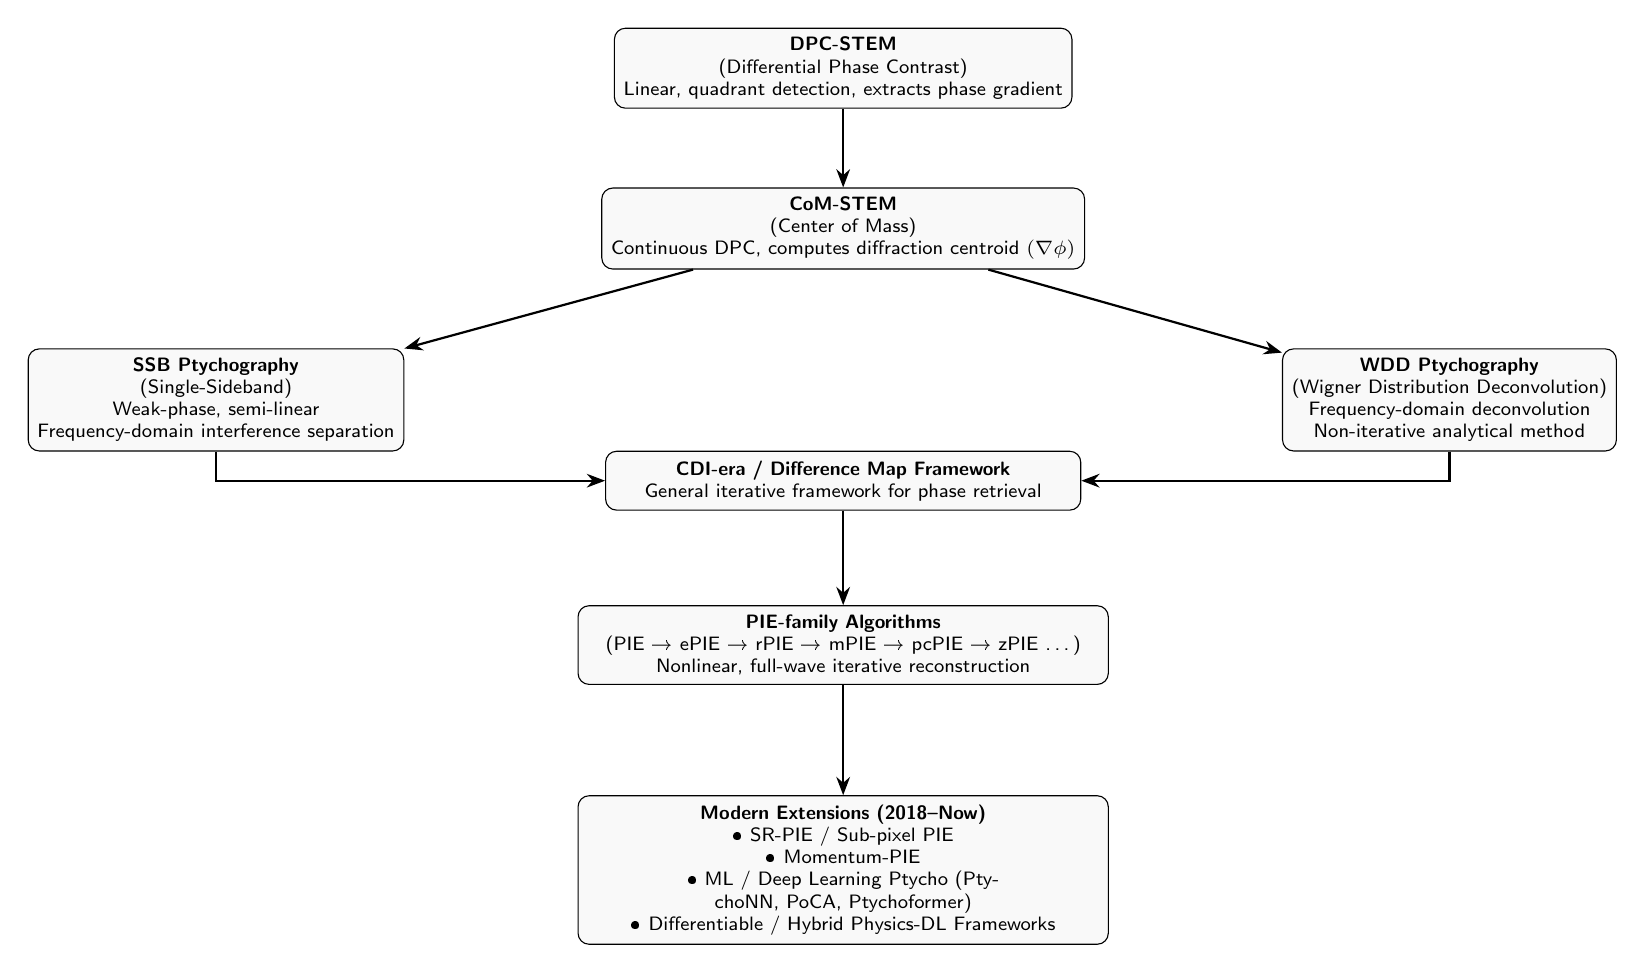
\begin{tikzpicture}[node distance=1.0cm, every node/.style={align=center, font=\scriptsize, rounded corners, draw, fill=gray!5}]


% Level 1
\node (dpc) {\textbf{DPC-STEM}\\(Differential Phase Contrast)\\Linear, quadrant detection, extracts phase gradient};


% Level 2
\node (com) [below=of dpc] {\textbf{CoM-STEM}\\(Center of Mass)\\Continuous DPC, computes diffraction centroid $(\nabla \phi)$};


% Level 3 - branches
\node (ssb) [below left=1.0cm and 2.5cm of com] {\textbf{SSB Ptychography}\\(Single-Sideband)\\Weak-phase, semi-linear\\Frequency-domain interference separation};


\node (wdd) [below right=1.0cm and 2.5cm of com] {\textbf{WDD Ptychography}\\(Wigner Distribution Deconvolution)\\Frequency-domain deconvolution\\Non-iterative analytical method};


% Connection to PIE family
\node (dm) [below=2.3cm of com, text width=5.8cm] {\textbf{CDI-era / Difference Map Framework}\\General iterative framework for phase retrieval};


\node (pie) [below=1.2cm of dm, text width=6.5cm] {\textbf{PIE-family Algorithms}\\(PIE → ePIE → rPIE → mPIE → pcPIE → zPIE …)\\Nonlinear, full-wave iterative reconstruction};


\node (modern) [below=1.4cm of pie, text width=6.5cm] {\textbf{Modern Extensions (2018–Now)}\\• SR-PIE / Sub-pixel PIE\\• Momentum-PIE\\• ML / Deep Learning Ptycho (PtychoNN, PoCA, Ptychoformer)\\• Differentiable / Hybrid Physics-DL Frameworks};


% Connections
\draw[->, thick] (dpc) -- (com);
\draw[->, thick] (com) -- (ssb);
\draw[->, thick] (com) -- (wdd);
\draw[->, thick] (ssb) |- (dm);
\draw[->, thick] (wdd) |- (dm);
\draw[->, thick] (dm) -- (pie);
\draw[->, thick] (pie) -- (modern);


\end{tikzpicture}}

\end{frame}



% ======================================================
\section{Algorithm Evolution (2004–2025)}
% ======================================================

\begin{frame}{Algorithm Evolution of the PIE Family (2004–2025)}
\scriptsize
\renewcommand{\arraystretch}{1.0}
\scalebox{0.8}{%
\begin{tabular}{p{2.5cm} p{3cm} p{4cm} p{3cm}}
\textbf{Stage} & \textbf{Representative Algorithms} & \textbf{Key Innovations} & \textbf{Mathematical Nature} \\
\hline
1 Early Iterative Engine (2004–2009) & PIE (Maiden \& Rodenburg, 2009, \textit{Ultramicroscopy}) & Introduced scan-overlap and error-reduction idea; single probe and strong phase approximation & Projection onto constraint sets (POCS) \\
2 Stabilization Phase (2009–2014) & ePIE, rPIE & ePIE: joint probe/object update; rPIE: proportional gain for high dynamic range & Gradient-descent-like (ADMM style) \\
3 Momentum and Robustness (2016–2018) & mPIE, SR-PIE, momentum-PIE & Added momentum, normalization, sub-pixel interpolation for faster convergence & Accelerated first-order optimization \\
4 Statistical Modeling (2018–2020) & ML-Ptychography (Odstrčil, 2018, \textit{Opt. Express}) & Replaced empirical error with explicit likelihood (Poisson noise model) & Maximum-likelihood estimation (MLE) \\
5 Mixed-state Modeling (2020– ) & Mixed-State ML-Ptychography (Chen et al., 2020, \textit{Nat. Commun.}) & Partial coherence modeling, multi-mode probes, mini-batch optimization & Probabilistic mixed-state + MLE \\
6 Learning-driven (2021–2025) & Neural-PIE, Deep Ptycho, PtychoNN, Ptychoformer & Deep learning for mapping updates and priors & Deep learning + Variational Bayesian optimization \\
\end{tabular}}
\vspace{6pt}

\textit{From linear models to hybrid Bayesian-learning frameworks, the PIE family evolved from physical iteration to differentiable inference.}
\end{frame}



% ======================================================
\section{Modern Research Lines}
% ======================================================

\begin{frame}{Three Major Research Lines (2020–2025)}
\small
\renewcommand{\arraystretch}{1.05}
\scalebox{0.8}{%
\begin{tabular}{p{3.5cm} p{5cm} p{5cm}}
\textbf{Line} & \textbf{Representative Work} & \textbf{Feature} \\
\hline
A. Physical Modeling Line & zPIE, Multi-slice PIE, Fresnel / Near-field, Partial Coherence & More accurate propagation and sample-thickness modeling; suited for physical realism \\
B. Statistical / Bayesian Line & ML-PIE, Mixed-State PIE, Variational Inference & Probabilistic noise and coherence modeling; mathematically grounded optimization \\
C. Neural Line & Neural-PIE, Ptychoformer, Deep Bayesian PIE & Fast, data-driven reconstruction; hybrid physics-learning design \\
\end{tabular}}
\vspace{8pt}


\end{frame}

% ======================================================
\section{Propagation Models and Geometry}
% ======================================================


\begin{frame}{Propagation Models in Electron Ptychography}
\begin{columns}
\column{0.55\textwidth}
\small
\begin{itemize}
\item \textbf{(A) Linearized models:} WPOA, Projection approximation.
\item \textbf{(B) Paraxial nonlinear:} Multislice propagation, partial coherence.
\item \textbf{(C) Full 3D / Nonparaxial:} Ewald curvature, dynamical diffraction, Bragg mode.
\end{itemize}
\column{0.45\textwidth}
%\includegraphics[width=\linewidth]{propagation_models.png}
\end{columns}
\vspace{4pt}
\textit{Key: Electron systems usually operate in quasi-Fresnel regime due to short $\lambda$ and limited z.}
\end{frame}
% ======================================================
\section{Maximum-Likelihood PIE}
% ======================================================

\begin{frame}{Maximum-Likelihood Ptychography (ML-PIE)}
\small
\textbf{Motivation:}  
Traditional PIE minimizes heuristic intensity error:
\[
E = \sum_j \|\,|\Psi_{\text{calc},j}| - \sqrt{I_{\text{meas},j}}\,\|^2
\]
which ignores detector noise statistics.  
ML-PIE instead derives its loss from the \textbf{Poisson noise likelihood:}
\[
p(I_{\text{meas}}|I_{\text{calc}})=
\frac{I_{\text{calc}}^{I_{\text{meas}}} e^{-I_{\text{calc}}}}{I_{\text{meas}}!}
\]

\textbf{Objective function (negative log-likelihood):}
\[
\mathcal{L}(O,P)=
\sum_{j,\mathbf{k}}
\bigl[I_{\text{calc},j}-I_{\text{meas},j}\ln I_{\text{calc},j}\bigr]
\]
\end{frame}

% ------------------------------------------------------

\begin{frame}{Iterative Update Scheme of ML-PIE}
\small
\textbf{1. Forward propagation:}
\[
\tilde{\Psi}_j = \mathcal{F}[\,P(\mathbf{r})O(\mathbf{r}-\mathbf{r}_j)\,], \quad
I_{\text{calc},j}=|\tilde{\Psi}_j|^2
\]

\textbf{2. Likelihood-based residual:}
\[
\Delta\tilde{\Psi}_j=
\frac{\tilde{\Psi}_j}{I_{\text{calc},j}}
\bigl(I_{\text{meas},j}-I_{\text{calc},j}\bigr)
\]

\textbf{3. Back propagation:}
\[
\Delta\Psi_j=\mathcal{F}^{-1}[\Delta\tilde{\Psi}_j]
\]

\textbf{4. Object \& probe update:}
\[
O^{(n+1)}=O^{(n)}+\frac{P^*(\mathbf{r})\Delta\Psi_j}{|P|^2+\epsilon},
\quad
P^{(n+1)}=P^{(n)}+\frac{O^*(\mathbf{r}-\mathbf{r}_j)\Delta\Psi_j}{|O|^2+\epsilon}
\]
\end{frame}

% ------------------------------------------------------

\begin{frame}{Advantages and Extensions}
\small
\textbf{Key advantages:}
\begin{itemize}
  \item Physically consistent with Poisson photon/electron counting noise.
  \item Naturally weights pixels by their signal strength (adaptive noise suppression).
  \item Provides stable convergence and high SNR reconstructions.
\end{itemize}

\textbf{Extensions:}
\begin{itemize}
  \item \textbf{Mixed-State ML-PIE:} adds multiple probe modes for partial coherence.
  \item \textbf{Bayesian / Variational PIE:} combines MLE with prior regularization.
\end{itemize}


\end{frame}






%============================================================
\section{Future Plan}
%============================================================
\begin{frame}{Plans for Next Week}
\footnotesize
\begin{itemize}
  \item [\ding{43}] Complete the study of electron dataset and do simulation of mixed-state ML-PIE in MatLab.
  \item [\ding{43}] Study the principle of maximum-likelihood PIE.
  \item [\ding{43}] Recalculate the algorithm from dpc to com, ssb and wdd ptychography.
\end{itemize}


\end{frame}



\end{document}
